\chapter{Introduction} \label{chap:intro}
\section{Why underwater?}
Manhood has managed to conquer variety of environments. At some point, humans could walk on the moon, send expeditions to cold or remote areas in different corners of the planet. Sea-bed embraces the largest part of the Earth's surface. Deep ocean world is a harsh environment with many discoveries yet to be revealed. Robots have potential to help in achieving those discoveries. 
\section{Localization - Where the Robot Is?}
One of the important features of the autonomous underwater vehicle is being capable of localising itself within an environment - to estimate its metric position and orientation in three dimensional space. Knowing where it actually is enables further tasks of an autonomous robot such as path tracking or various manipulation tasks. Therefore, it has the same role as parts of human brain devoted to navigation.  

The main topic of the thesis is localization of an autonomous underwater vehicle. Localization essentially deals with the problem of estimation of the position and orientation of the vehicle with respect to a defined reference. Simply, answering where the robot is. Basic instrument in accomplishing the localisation is the sensor set. Sensory system is used to give the feedback on vehicle movement, control or state of the surrounding environment. One of the difficulties of such process is the nature of the measurement, mostly based on distance evaluation in water environment, noise and uncertainty of the sensing process. 

The idea is to establish the matching between the sensor measurements and the location attained. This process is not straightforward since many conditions influence the performance, including the very beginning of the localization: whether we have some previous estimate on the position or not \cite{ribas10}. 

%Localization can alternatively be carried out by analysing the pose possibilities and choosing the one that better correlates to measurements or the map. Such methods are Monte Carlo localization and Markov localization. The other approach, a set of hypotheses for coupling together the sensor measurements and the map features. These hypotheses are ranked depending on number of consistent matches where the one with highest ranking is defining the position. This can be a costly process, therefore a number of methods deals with optimization of it. 
\section{Autonomous underwater vehicle (AUV)}
Different sorts of underwater robots have been developed throughout recent decades of research. They all have various performance capabilities, costs, accuracy, power consumption characteristics. The algorithm presented in this thesis was applied on Ocean System Lab's (web link???) torpedo-shaped Nessie vehicle (figure ~\ref{fig:nessie6}) that belongs to special-task AUV category \cite{bahr08} combining together FOG-based Inertial Navigation System, DVL and LBL sensoring for navigation (Chapter ~\ref{chap:sensors}). The architecture of the vehicle and its system capabilities are flexible on number and types of sensors employed which leaves space for additional equipment to assist in missions, or improve the current navigation with already existing devices, such as forward or downward looking cameras. 

\begin{figure}%[htp]
\centering
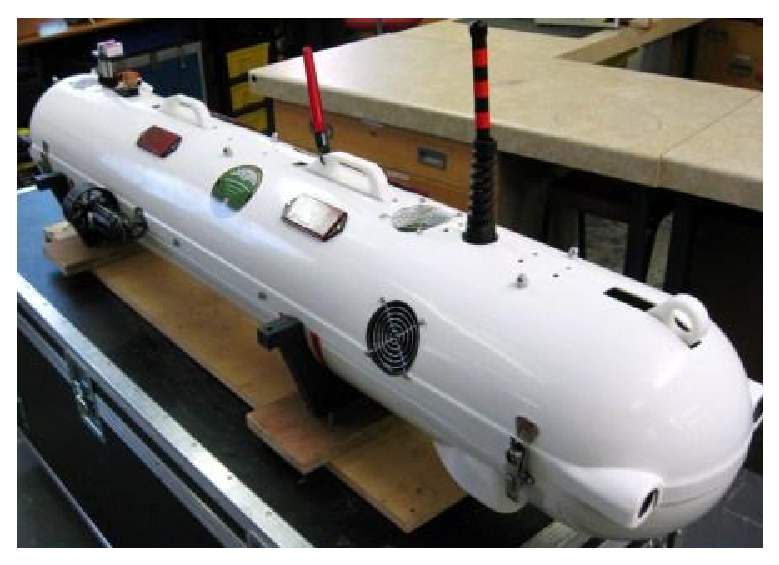
\includegraphics[width=0.5\linewidth]{intro/fig/nessie6.eps}
\caption{Nessie VI design.}
\label{fig:nessie6}
\end{figure} 

\section{Contribution of the thesis}
Thesis is reporting application of Extended Kalman filter for localization in unstructured environment of an AUV described in previous section. The concept of sensor fusion was explained. Idea of blending together sensor measurements can be exploited in different situations. Purpose is to demonstrate its application on a real underwater vehicle, report advantages, disadvantages. Apart from algorithm level, work examines the problem from the perspective of the matter - how to make a successful AUV navigation. 
\section{Thesis outline}
....
%%\subsection{Paper}
%%The manuscript should be in A4 size, and the printed paper should
%%be of at least 70 gsm.
%%
%%\subsection{Font and margins}
%%Thesis should be printed on both sides of the paper. Use no less
%%than 1.5 spacing, with quotations and notes single-spaced.
%%Regarding \textbf{Character size}, not less than 2.0mm for
%%capitals and 1.5mm for x-height (the height of a lower-case x). Us
%%a serif font (i.e. Times) between 10 and 12 points. Use consistent
%%and clear fonts through all the document.
%%
%%The text layout should be approximately as follows:
%%
%%\begin{itemize}
%%    \item $4cm$ binding margin
%%    \item $2cm$ head margin (top of page)
%%    \item $2.5cm$ fore-edge margin
%%    \item $4cm$ tail margin (bottom of page)
%%\end{itemize}
%%
%%\section{Title Page}
%%The title page should contain the title of thesis, authors name,
%%and at the foot of the page: the name of degree,  Your University,
%%and the year of presentation. Something like this:
%%
%%\vspace*{1cm}
%%\begin{center}
%%{\Large\bf MSc. Thesis example VIBOT\\} \vspace{2cm} {\large
%%Robert Mart\'i\\
%%\vspace{1cm}
%%Department of Computer Architecture and Technology \\
%%University of Girona}
%%
%%\end{center}
%%
%%\vspace{2cm}
%%\begin{center}
%%{\large A Thesis Submitted for the Degree of MSc Erasmus Mundus in
%%Vision and Robotics (VIBOT)\\ \vspace{0.3cm} $\cdot$ 2008 $\cdot$}
%%\end{center}
%%
%%
%%\subsection{References}
%%You can reference other authors by using the $cite command$
%%\cite{Pokorski:1998hr}. You are encouraged to use bib files and
%%let bibtex do the job for you.
